\documentclass[a4paper]{article}

\usepackage[utf8]{inputenc}

\usepackage{enumitem}

\usepackage{url}
\usepackage{hyperref}
\hypersetup{
    colorlinks=true,
    linkcolor=blue,
    filecolor=magenta,      
    urlcolor=cyan,
}
\usepackage{caption}

\usepackage{listings}
\lstset{basicstyle=\ttfamily,
  showstringspaces=false,
  commentstyle=\color{red},
  keywordstyle=\color{blue},
  captionpos=b,
  breaklines=true
}

\usepackage{color}

% *** GRAPHICS RELATED PACKAGES ***
%\usepackage[pdftex]{graphicx}
\usepackage{graphicx}
%\usepackage[dvips]{graphicx}
% to place figures on a fixed position
\usepackage{float}

\usepackage[margin=1in]{geometry}

\title{Blockhain Tutorial}
\author{}
\date{}


\begin{document}

\maketitle

\tableofcontents

\section{Introduction}

Introduce this tutorial : topics discussed, high-level overviewe of the excersises

\section{Blockchain concepts,basiscs}

desrcibe main concepts of Blockchain 

The introduction to Mininet, OpenFlow and POX controller can be read in the
\href{https://qosip.tmit.bme.hu/foswiki/pub/Meres/OpenFlowMSc/OpenFlow-Mininet-syllabus-en.pdf}{OpenFlow \& Mininet
    syllabus}. On
Figure~\ref{fig:Lab-topo} the network topology used in this P2P lab is shown.


\begin{lstlisting}[language=python,frame=single,breaklines]
packet = event.parsed  
\end{lstlisting}


\section{Smart contracts}


\section{Smart contracts using Ethereum}


\section{Introduction to the demo environment}

The following tools are \textbf{required} in order to effectively participate in the tutorial
\begin{itemize}
    \item Web browser supporting ECMAScript 2015
    \item SSH client (e.g. \emph{putty} on windows, \emph{openssh} on linux
    \item Arbitrary text editor for Solidity smart contract editing
\end{itemize}{}

The \href{https://blockchain.cnsm2019-tutorial.com/}{demo environment} - as illustrated by Figure \ref{fig:demo-env} - consists of a Web UI and back-end for managing the training sessions and allowing that the participants can easily interact with each other's deployed contracts.The back-end interacts with the Etherum based blockchain network using web3 API. The blockchain network consists only one node for now, but that doesn't greatly affects how the endpoints would interact with the blockchain network as long as connection is available to a node.

\begin{figure}[H]
    \centering
    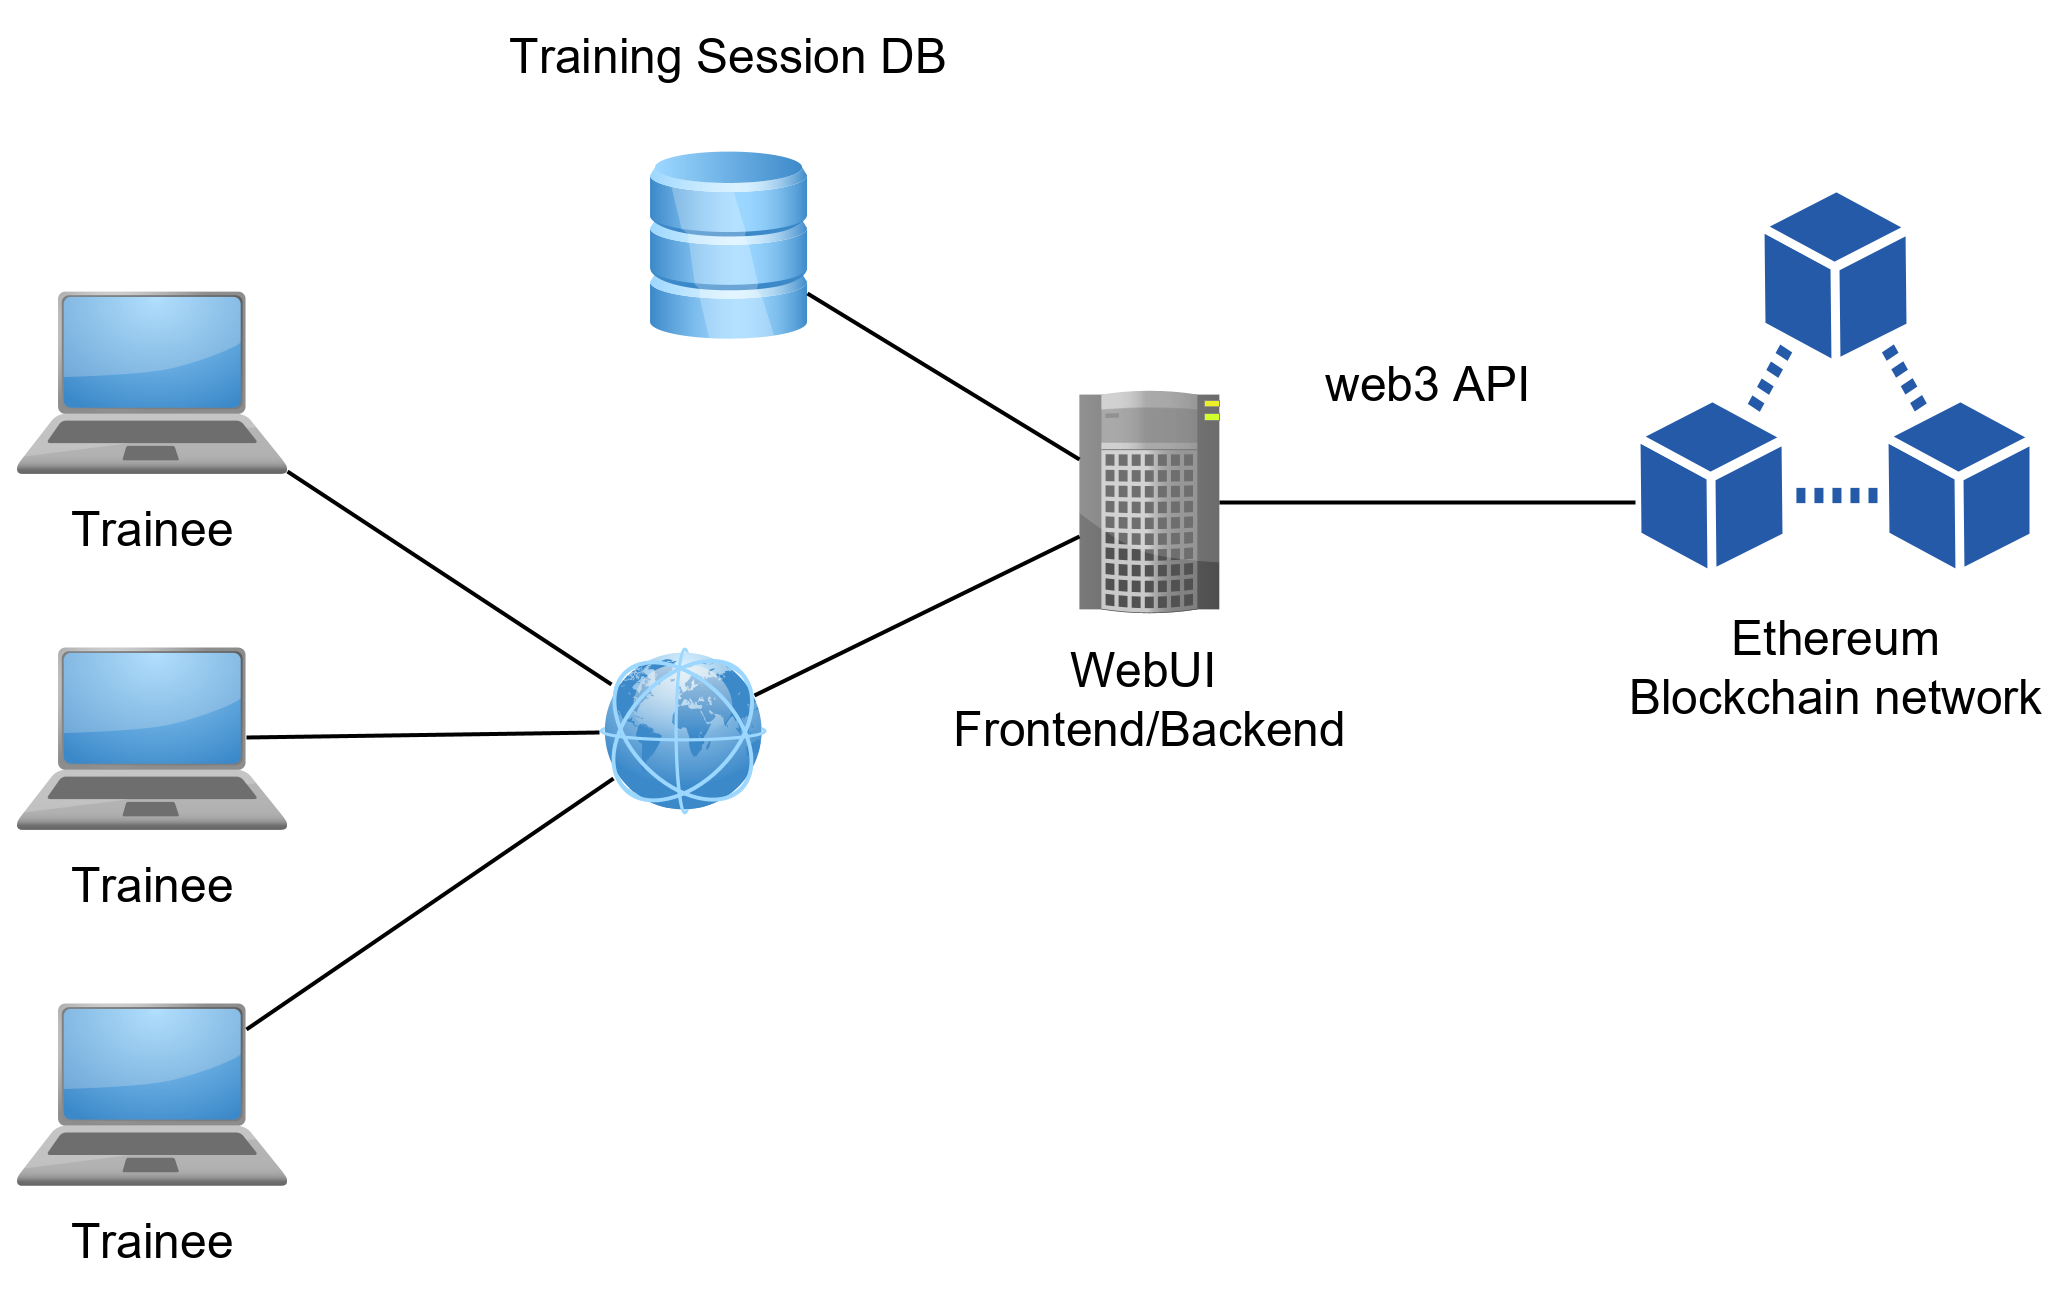
\includegraphics[width=0.9\textwidth]{figures/env.png}
    \caption{The tutorial environment}
    \label{fig:demo-env}
\end{figure}

Registration is available, but at the beginning of the hands-on part of the tutorial the participants will receive usernames and passwords to use as that accounts will be pre-filled so that contract deployment can be performed right away.

For using the \texttt{geth} console the participants are expected to be able to login to \url{ssh://tutorial@blockchain.cnsm2019-tutorial.com:2222} i.e. SSH using port \textbf{2222} and using username \texttt{tutorial} to host \url{blockchain.cnsm2019-tutorial.com}. The password to be used will be provided during the tutorial session.

\section{Tutorial exercises}

\subsection{Verify logins}

\begin{enumerate}[label=\textbf{Task \arabic*}:, series=l_tasks]
\item login both to the WebUI and to the backend host using ssh.
\end{enumerate}

After logging in to the web page, you should see your etherum account in the top portion of the screen(see Figure \ref{fig:login-user-acc}). After this step verify that you are able to log in using ssh to the back-end.

\begin{figure}[H]
    \centering
    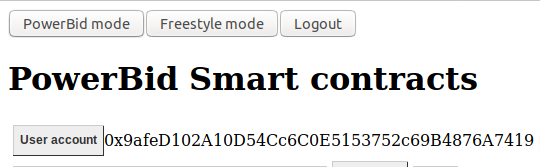
\includegraphics[width=0.9\textwidth]{figures/login-useracc.png}
    \caption{Displayed user account}
    \label{fig:login-user-acc}
\end{figure}

\begin{enumerate}[label=\textbf{Task \arabic*}:,l_tasks]
\item Check your balance using the \texttt{geth} node in console mode using commands found in listings \ref{lst:attach} and \ref{lst:balance}
\end{enumerate}

\begin{lstlisting}[language=bash,caption={attach to geth node},label={lst:attach}]
sudo ./admin/geth_attach 
\end{lstlisting}

\begin{lstlisting}[language=javascript,caption={Function for checking balance},label={lst:balance}]
eth.getBalance(account)
\end{lstlisting}

You should see a number greater than 0. The \textttt{geth} console is a javascript REPL and essentially the commands that can be used are the ones the web3 API exposes. For further reference of functions please study the corresponding \href{https://web3js.readthedocs.io/en/v1.2.1/web3.html}{web3 API documentation}.


After successful execution something similar shoud be seen:
\begin{verbatim}
tutorial@87cd2f75a465:~$ sudo ./admin/geth_attach 
[sudo] password for tutorial: 
Welcome to the Geth JavaScript console!

instance: Geth/v1.9.1-stable-b7b2f60f/linux-amd64/go1.12.7
coinbase: 0xf5573ac8504e8280c43806c156ff52984bc35c16
at block: 1133 (Sun, 13 Oct 2019 10:08:50 UTC)
 datadir: /iot_sc_tutorial/datadir
 modules: admin:1.0 debug:1.0 eth:1.0 ethash:1.0 miner:1.0 net:1.0 personal:1.0 rpc:1.0 txpool:1.0 web3:1.0

> eth.getBalance("0x9afeD102A10D54Cc6C0E5153752c69B4876A7419")
1e+22
> 
\end{verbatim}

As one can notice this \textttt{eth.getBalance} function returns the balance in \emph{Wei}. There's a utility function called \textttt{web.toWei} in the web3 module which can be used to transform between units e.g. to get the balance in \emph{ether} the following can be executed:
\begin{verbatim}
> eth.getBalance("0x9afeD102A10D54Cc6C0E5153752c69B4876A7419")/web3.toWei(1,"ether")
10000
> 
\end{verbatim}



\subsection{Transactions using the console}

As a next step we will initiate transactions using the geth console.

\begin{enumerate}[label=\textbf{Task \arabic*}:,l_tasks]
\item Select one of your peers as recipient and transfer 1 ether to them using the console. Check your balance before and after the transaction. The corresponding function to use is \ref{lst:balance} and \ref{lst:transfer}
\end{enumerate}

\begin{lstlisting}[language=javascript,caption={Functions to be used for signing and sending a transaction},label={lst:transfer}]
signedTranaction = personal.signTransaction({
    from: '0x9afeD102A10D54Cc6C0E5153752c69B4876A7419',
    to: '0x3FecF304285303Fba1C34124889Ea1256e9BB0de',
    value: web3.toWei(1,"ether")
    gas: 200000, 
    gasPrice:eth.gasPrice,
    nonce: eth.getTransactionCount("0x9afeD102A10D54Cc6C0E5153752c69B4876A7419")
    }, "user1")


transactionId = eth.sendRawTransaction(signedTranaction.raw)

eth.getTransaction(transactionId)
\end{lstlisting}

It could be that initial result of the transaction data might not contain the block hash and block number as it is in pending. In such case repeat the \textttt{eth.getTransaction(transactionId)} command until those fields are populated

\begin{enumerate}[label=\textbf{Task \arabic*}:,l_tasks]
\item Analyze the block that contains your previous transaction, and check which other transactions might reside in the same block as yours using the commands in listing \ref{lst:block}
\end{enumerate}

\begin{lstlisting}[language=javascript,caption={Functions for analyzing a block},label={lst:block}]
eth.getBlock(eth.getTransaction(transactionId).blockNumber)

eth.getBlock(eth.getTransaction(transactionId).blockNumber).transactions.map(function(tx){return eth.getTransaction(tx);})
\end{lstlisting}

\subsection{PowerBid game}

As part of familiarizing ourselves with the concepts of smart contracts and their potential use cases in IoT environments we are going to use a game. The game consists of a pre-implemented and simple smart contract that is modelling an electrical power auction. The has 2 roles: supplier and consumer. The contract is created by the consumer where he specifies the required energy and the approximate time window where he intends to consumed the required power. He also specifies a maximum price to pay for this amount of energy at that time window. The suppliers essentially then monitor these contracts whether they can satisfy them while maximizing their profit the bid accordingly. This model is a sell auction i.e. a smaller price is considered more aggressive. 

The contract has been described in Solidity language and it's current source that is used during this tutorial can be studied \href{https://raw.githubusercontent.com/fecjanky/iot_sc_tutorial/v1.0.4/src/powerbid.sol}{here}.

The contract has the following main states:
\begin{enumerate}
    \item Auction Phase, where the suppliers participate in the sell auction
    \item Consumption Phase, where the consumer consumes the power paid and requested
    \item Withdraw Phase, where the consumer can withdraw his gain (that is the difference between the max. price and the best price) and the supplier can withdraw the funds from the contract
\end{enumerate}



\begin{figure}[H]
    \centering
    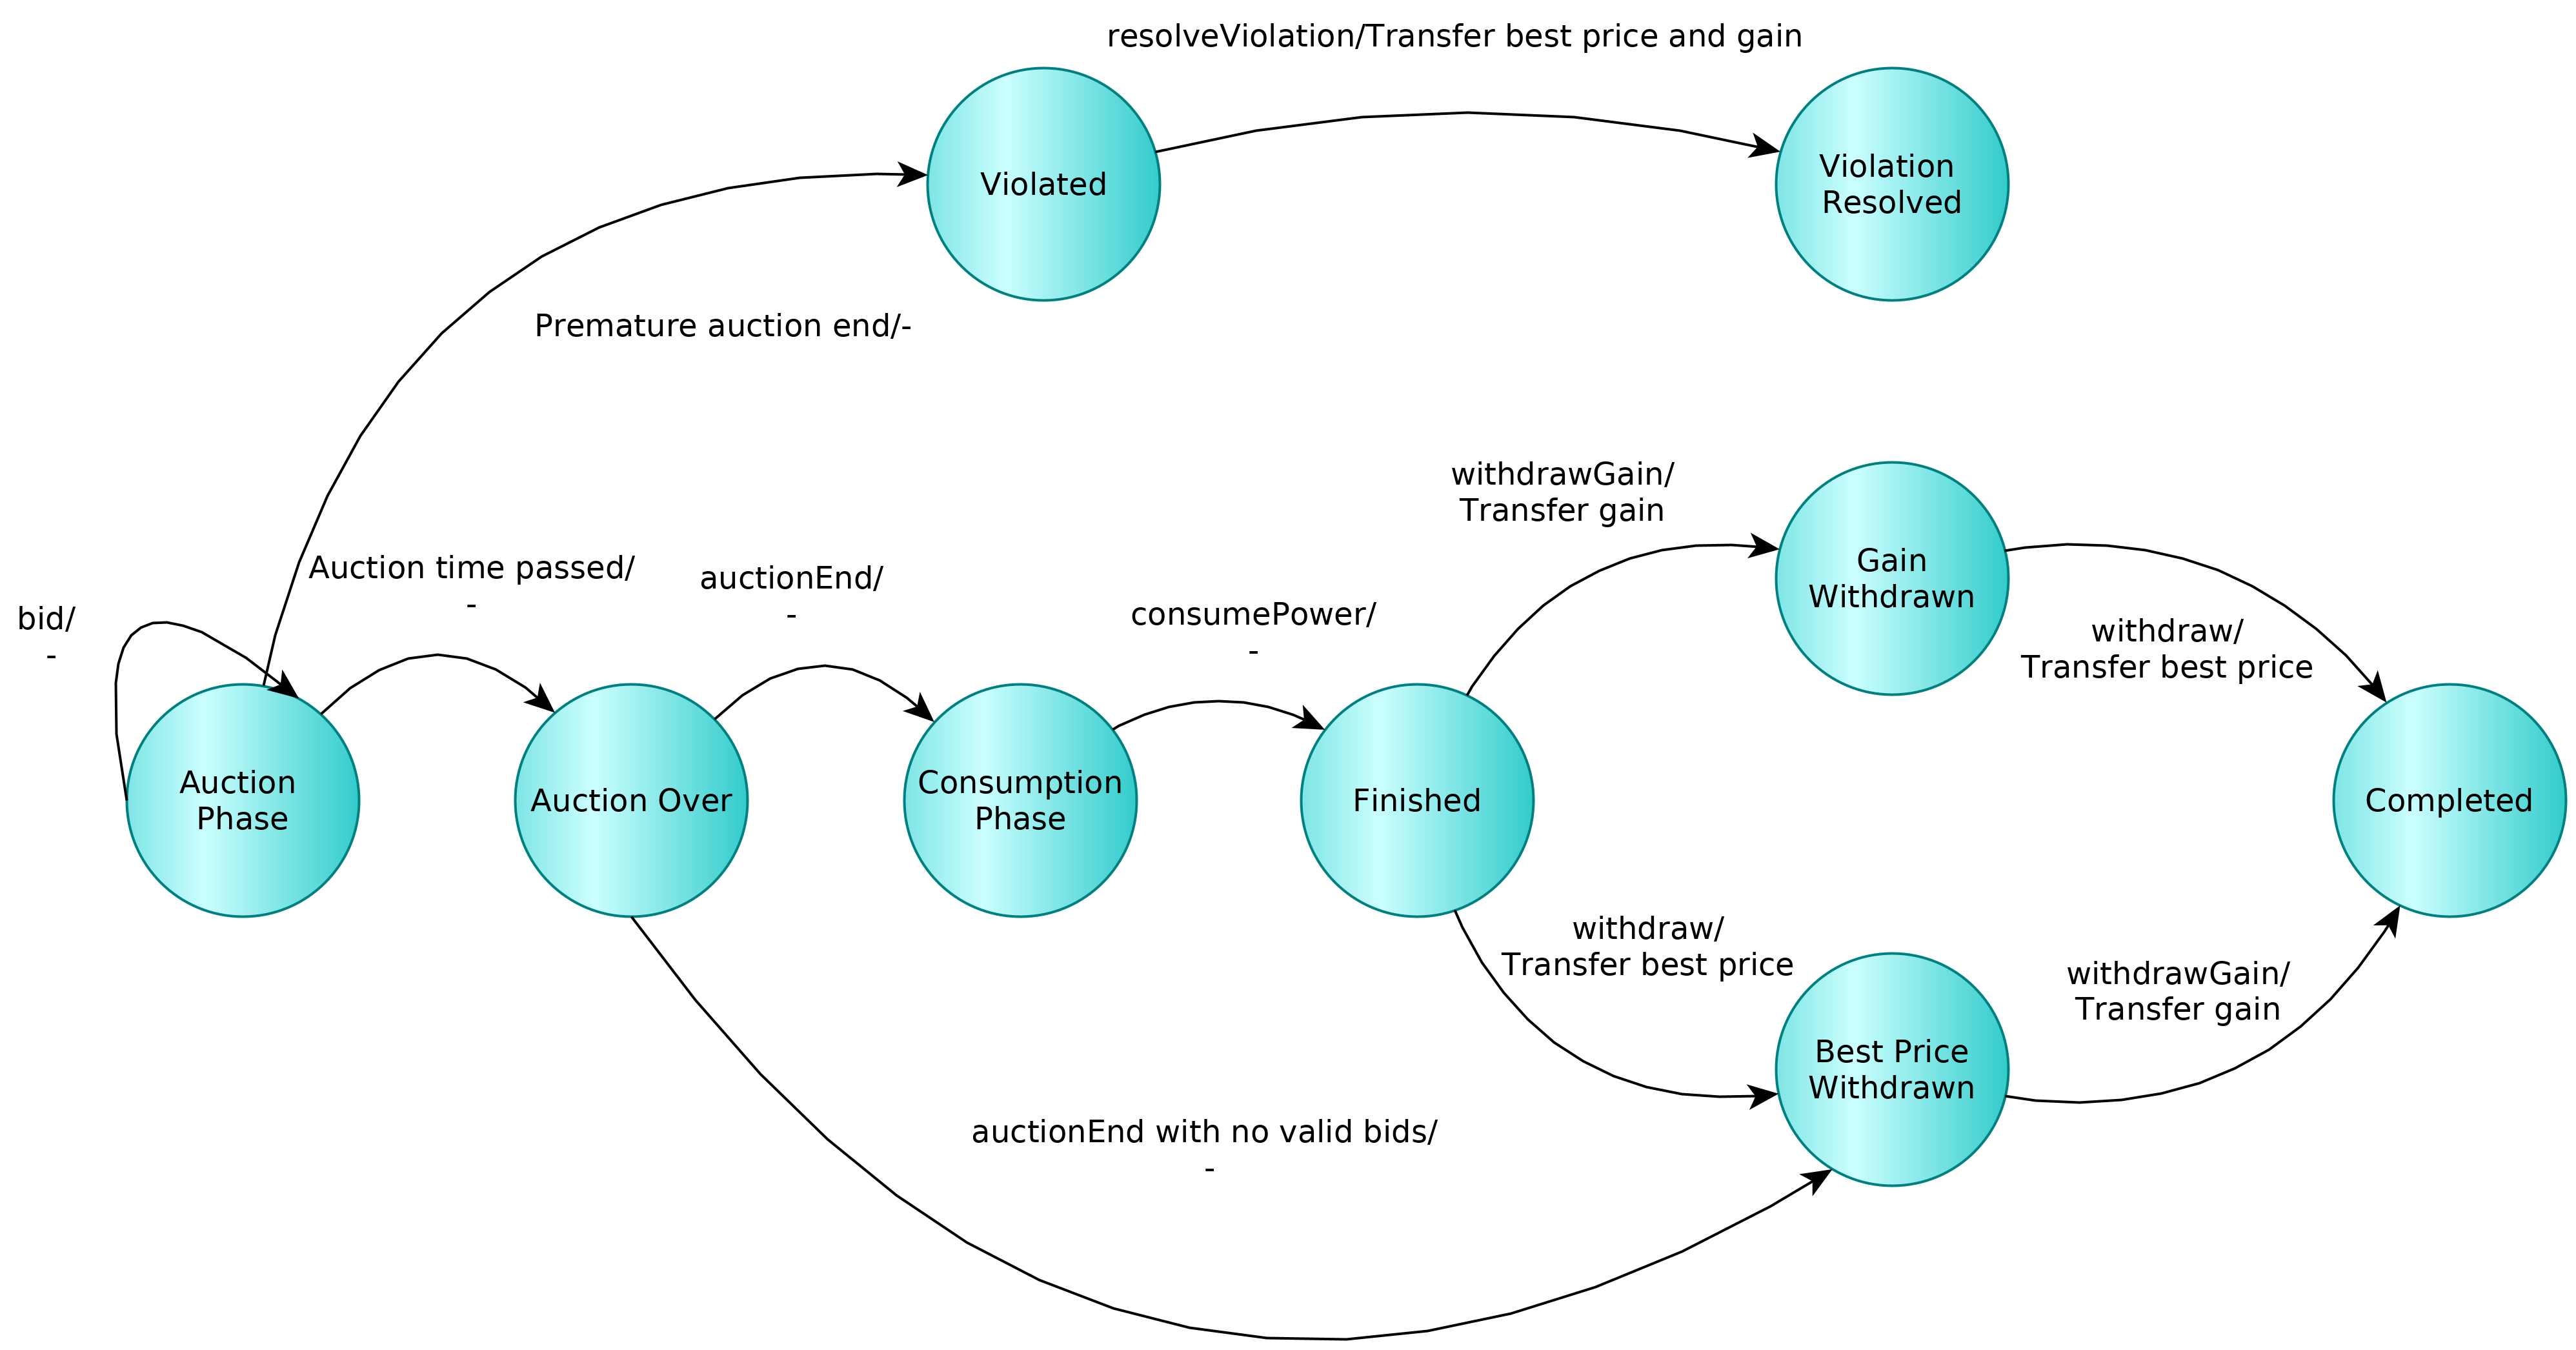
\includegraphics[width=0.9\textwidth]{figures/state_diagram.png}
    \caption{The state diagram of the PowerBid smart contract}
    \label{fig:State-diagram-powerbid}
\end{figure}


\subsection{Implement a number guessing game}

\end{document}